\section{Blobs and holes}
\cref{sec:blobsAndHoles}
%
The aim of this chapter is to characterize the intermittent structures observed in the time traces in \cref{fig:combinedPlots008} by using a conditional averaging (CA) technique.
It turns out that the intermittent structures shares characteristics with what has been described as blobs in the literature.
We will here use the definition of a blob given in the review paper by D'Ippolito et. al. \cite{DIppolito2011}.
In this definition, a blob is a structure which satisfies the following properties:
%
\begin{quote}
    \begin{enumerate}[noitemsep]
            \item  it has a monopole (single-peaked) density distribution with a peak value much higher than the surrounding rms fluctuations of the background plasma (typically $\geq 2-3$ times higher);
            \item  it is aligned parallel to the magnetic field $B$ and its variation along $B$ is much weaker than in the transverse direction, i.e., $\delta/L_\|\ll1$;
            \item it has a dominant convective $\ve{E}\times\ve{B}$ velocity component in the direction of a charge-polarizing force, and an associated potential and vorticity with a dipole structure in the direction transverse to its propagation.
    \end{enumerate}
\end{quote}
%
Usually, the blobs observed in tokamaks are driven by magnetic field inhomogenities through the so-called grad-$B$ drift.
This drift is causing a polarization, and the polarization are driving the blobs outwards through the $\ve{E}\times\ve{B}$ drift.
The blobs in tokamaks are therefore self-propelled, and does not depend on local gradients of the plasma \cite{Krasheninnikov2008}.

\subsection{The conditionally averaging technique}
%
The CA technique is often used to tell something about the average of coherent structures in turbulence.
It has it roots in fluid dynamics \cite{Kovasznay1970}, with the first application to plasma physics in \cite{Huld1990}. Although improvements to the original technique has been done for for example noisy data recorded with a probe \cite{Teliban2007}, we will use the simple, classic variant of the technique here:
%
\begin{algorithm}
\begin{enumerate}[noitemsep,nolistsep]
    \item Record a signal in a single point over time.
    \item Set a threshold condition.
    \item When the signal reaches the condition, record a sub-signal $\tau$ time units before and $\tau$ time units after.
        The recorded sub-signal will be one of the samples in the conditional averaging.
    \item Take the average of all the samples, i.e. the recorded sub-samples.
\end{enumerate}
\end{algorithm}
%
Here, we will set the threshold condition on the radial flux.
Alternatively, we could have set a condition on the perturbation in $n$ itself.
This would have the disadvantage of including samples of perturbation which arises from poloidal rotation of a slightly elongated plasma.
In the end we are interested in structures which "has a dominant convective $\ve{E}\times\ve{B}$ velocity component" from point $3$ in the definition given in \cref{sec:blobsAndHoles}.

\subsection{The averaged structures}
The time trace of the radial flux, together with three different conditions are shown in \cref{fig:blobFluxTT}.
%
\begin{figure}[htb]
    \begin{center}
        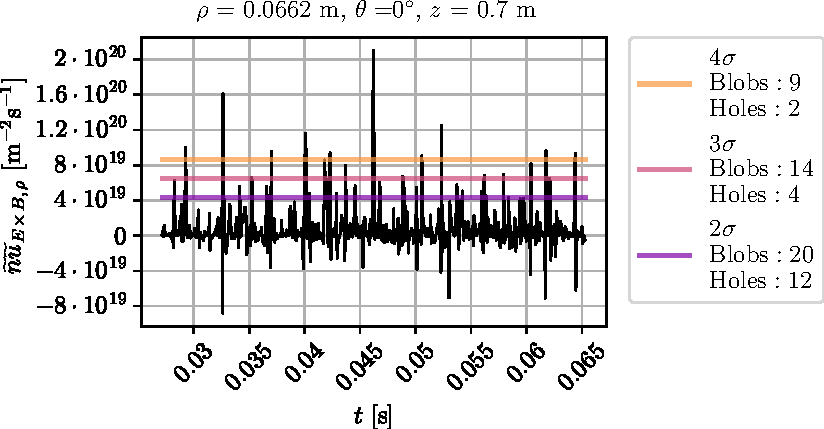
\includegraphics{fig/results/blobs/blobFluxTimeTrace_B0_008Tweak}
    \end{center}
    \caption{
        Time trace of the flux for $B=0.08\T$.
        The trigger conditions for $2\sigma$, $3\sigma$ and $4\sigma$ is indicated on the figure, and the number of events found are indicated in the legend.
    }
    \label{fig:blobFluxTT}
\end{figure}
%
Is apparent that the trigger signal is highly intermittent, as seen from the PDF in \cref{fig:blobFluxPDF}, which shows a skewness of approximately $3$, and an excess kurtosis of around $16.7$.
%
\begin{figure}[htbp]
    \centering
    \begin{subfigure}[h]{0.45\textwidth}
        \center
        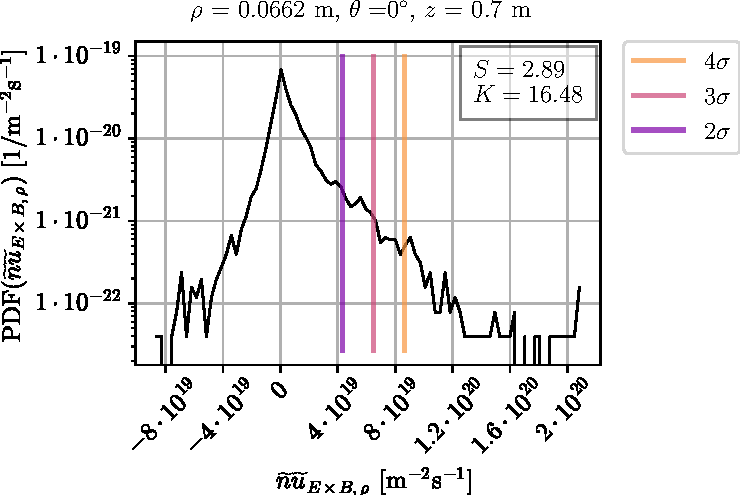
\includegraphics{fig/results/blobs/blobFluxPDF_B0_008Tweak}
        \caption{The PDF of the radial flux.}
        \label{fig:blobFluxPDF}
    \end{subfigure}
    \hfill
    \begin{subfigure}[h]{0.45\textwidth}
        \center
        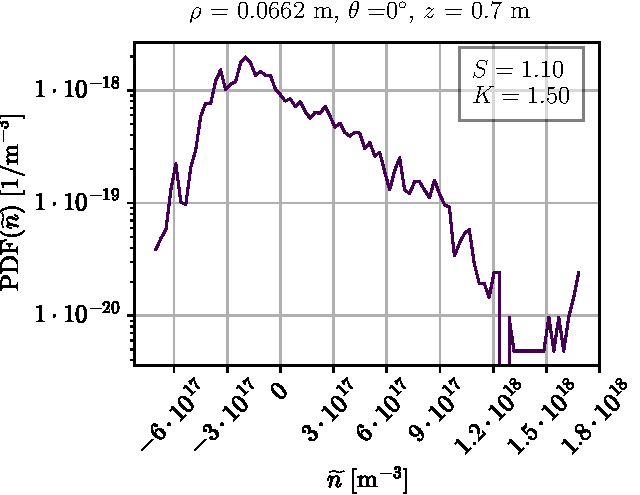
\includegraphics{fig/results/blobs/blobDensPDF_B0_008Tweak}
        \caption{The PDF of the density.}
        \label{fig:blobDensPDF}
    \end{subfigure}%
    \caption{PDFs of the radial flux and the density measured in the same point as \cref{fig:blobFluxTT} for $B=0.08\T$.
            $S$ indicates the skewness and $K_E$ the excess kurtosis.}
\end{figure}
%

We now chose the time window parameter $\tau$ to be $4$ times the time of the maximum pulse duration (where the signal is above the threshold) of the flux%
\footnote{Note that it is usual to set $\tau$ to the autocorrelation time of the signal.
    However, as we would like to sample the densities given the trigger signal on the flux, we make the somewhat arbitrary choice of $\tau$.
}%
.
From the flux signal we can now extract the times where the condition is met its corresponding time window.
This can be used to sample any quantity in any spatial point.
In other words, we can use these time to conditionally sample the density $n$ to search for blobs.
Before doing so, we note that we are dealing with two types of events, both giving a positive radial flux.
The events can either be:
%
\begin{enumerate}[noitemsep]
    \item A blob: A positive perturbation propagating in positive $\rho$.
    \item A hole: A negative perturbation propagating in negative $\rho$.
\end{enumerate}
%
The time trace of the CA structures of both blobs and holes are shown together in \cref{fig:blobAndHoleTT}.
%
\begin{figure}[htb]
    \begin{center}
        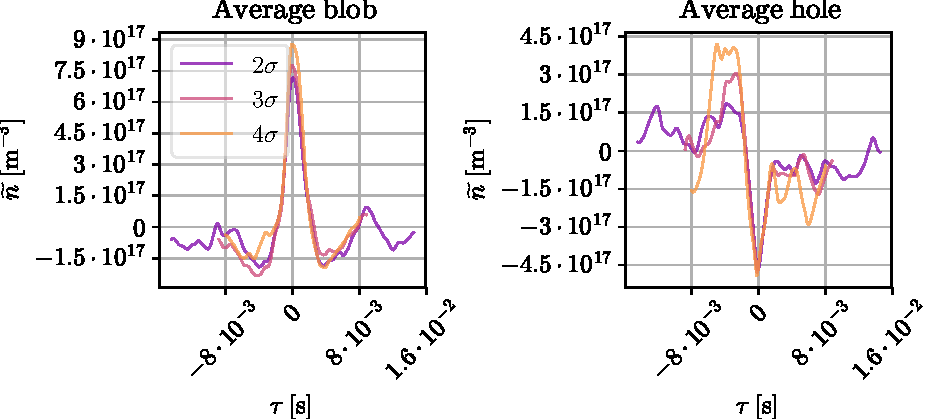
\includegraphics{fig/results/blobs/blobsAndHoles-B0_008Tweak}
    \end{center}
    \caption{The averaged blob and hole density structures for $\rho=0.0662\m,\;\phi=0^{\circ}\;z=0.7\m\;B_0=0.08\T$ found when using the trigger signal in \cref{fig:blobFluxTT}.}
    \label{fig:blobAndHoleTT}
\end{figure}
%
Note that the amplitude of the blobs and the holes are relatively insensitive to the choice of the condition.
If we would set a condition on the same variable as we took the conditional average of, we would for a Gaussian white noise process have the relation \cite{Edwards1983}
%
\begin{align*}
    \innp{\wt{a}}{a_*} = a_*R(\wt{a}),
\end{align*}
%
where we have used the notation
%
\begin{align*}
    \text{Conditional average} = \innp{\text{Signal to average}}{\text{Trigger value}},
\end{align*}
%
and where $R(\wt{a})$ denotes the normalized correlation function given by
%
\begin{align*}
    R(\wt{a}) = \frac{(\wt{a}\star\wt{a})}{\expt{\wt{a}^2}_t}.
\end{align*}
%
However, it is unclear if the same holds when the CA is performed for $\innp{n}{\Gamma_*}$ as the term contains a tripple correlation%
\footnote{One could find out if the relation holds by generating a random synthetic signal of pulses of $\wt{n}$ and $\wt{\ve{u}}_{E\times B, \rho}$ and pack the pulses close enough together in order to make the signal Gaussian \cite{PecseliPrivate}}%
.

One could be tempted to state that since the flux signal in \cref{fig:blobFluxPDF} is not Gaussian, the denisty signal must also be non-Gaussian, so we can conclude that the density signal is a result of coherent structures in the plasma, rahter than an artifact of the conditional sampling technique.
However, even if the both the PDF of the density fluctuations and the PDF of the $\ve{u}_{E\times B,\rho}$ fluctuations were Gaussian the product would not be Gaussian as shown in \cite{Bergsaker2015}.

In order to tell if our structures are a consequence of Gaussian random noise, we must therefore look at the PDF of the density signal.
The PDF of the density is shown in \cref{fig:blobDensPDF}.
With its skewness around $1$ and an excess kurtosis of about $1.5$ is not as intermittent as the radial flux, nor is it a Gaussian random process.
%

Instead of sample the density at the same point as the condition is set, we can sample the whole perpendicular plane for the density fluctuations.
Such a sample can also be made in experiments (under the assumtions that the experiments are reproducible) by fixing one probe for the triggering signal, and sweep another probe through the perpendicular plane, as done in for example \cite{Nielsen1996}.
The result is shown in \cref{fig:perpBlob008}.
%
\begin{figure}[h!]
\begin{tabular}{ccc}
  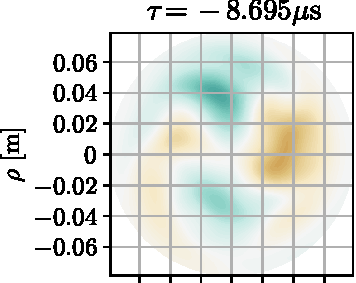
\includegraphics{fig/results/blobs/matrix-perp-blobs-B0_0.08-fluct/0} &
  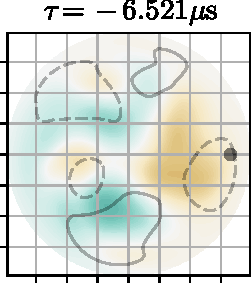
\includegraphics{fig/results/blobs/matrix-perp-blobs-B0_0.08-fluct/1} &
  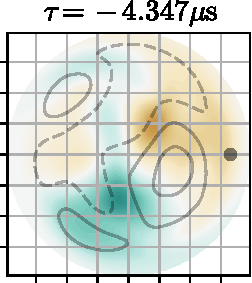
\includegraphics{fig/results/blobs/matrix-perp-blobs-B0_0.08-fluct/2} \\
  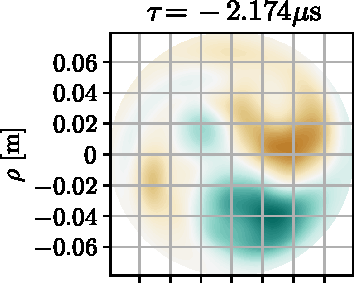
\includegraphics{fig/results/blobs/matrix-perp-blobs-B0_0.08-fluct/3} &
  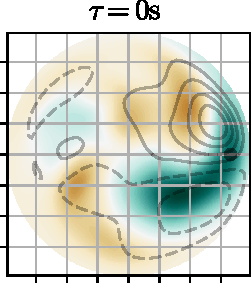
\includegraphics{fig/results/blobs/matrix-perp-blobs-B0_0.08-fluct/4} &
  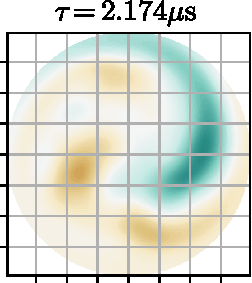
\includegraphics{fig/results/blobs/matrix-perp-blobs-B0_0.08-fluct/5} \\
  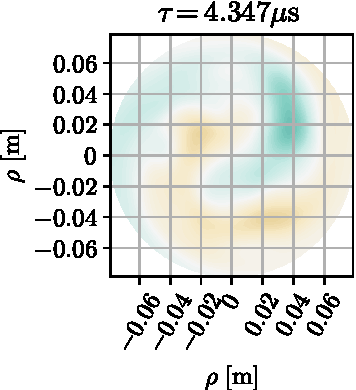
\includegraphics{fig/results/blobs/matrix-perp-blobs-B0_0.08-fluct/6} &
  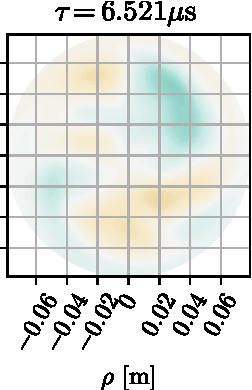
\includegraphics{fig/results/blobs/matrix-perp-blobs-B0_0.08-fluct/7} &
  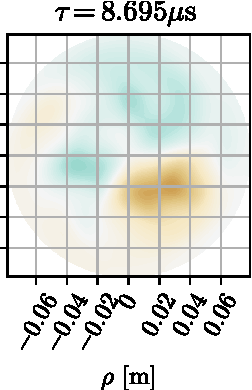
\includegraphics{fig/results/blobs/matrix-perp-blobs-B0_0.08-fluct/8} \\
  \multicolumn{3}{c}{\hspace*{2cm}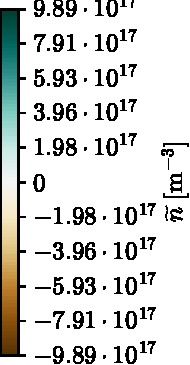
\includegraphics[angle=-90]{fig/results/blobs/matrix-perp-blobs-B0_0.08-fluct/colorbar}}
  \\
\end{tabular}
\caption{Perpendicular snapshot of a conditionally averaged blob at $z=0.7\m$ for $B=0.08\T$.
    The colormap represents the density fluctuations,
    the contour lines represents the potential, whilst the black dot denotes the position where the trigger signal for radial flux is set to $3\sigma$.
}
\label{fig:perpBlob008}
\end{figure}
%
Although we are setting the condition at the flux at $\theta = 0$, we can see that the blob start to form around $\theta = 3/2 \pi$ at $\tau=-4.347\mu \s$.
The structure gets an associated potential dipole structure, which transports the structure radially outwards through the $\ve{E}\times\ve{B}$-drift.
As the time evolves, the structure is also transported in the ion diamagnetic direction by the background flow set up by the background vorticity as shown in \cref{fig:radProfs}.
As the structure is transported radially outwards, it enters region with increasing background poloidal shear.
This elongates the structure as seen at $\tau=2.147\mu \s$.
After the shearing of the structure only background noise of the density and potential remains at $\tau \geq4.347\mu \s$.

One can now pose the question:
"What mechanism is creating the associated potential dipole structure of the monopole density structure?".
Obviously we have set the sampling condition on the radial flux, so the dipole structure may not be surprising.
However, in blobs seen in tokamaks, the polarization of charge can be explained through the curvature and $\grad B$-drift.
If we let $\ve{v}_\a$ denote the particle velocity for species $\a$, these drifts are given by%
\footnote{For the equivalent drift in the fluid picture, see \cite{Garcia2003}.}
%
\begin{align}
    \ve{v}_{\mathcal{C},\a} + \ve{v}_{\grad B,\a} = \frac{m v_{\a,\perp^2}}{2q_\a B^2}\ve{b}\times\grad B + \frac{m v_{\a,\|^2}}{q_\a B}\curl\ve{b},
    \label{eq:chargeSep}
\end{align}
%
where the charge separation comes about as $q_\a$ has opposite sign for electrons and ions.
As the $B$ field is homogeneous in our case, the drifts in \cref{eq:chargeSep} cannot be the cause of the charge separation.
Another possible candidate for the charge separation is the neutral wind, which gives rise to a charge separation through a differences in the neutral temperatures \cite{Krasheninnikov2003}.
However, as the plasma in the simulations presented in this chapter is fully ionized (i.e. no neutrals), we can rule out the neutral wind as a candidate for the charge separation.

A possible candidate for the charge separation is the Kelvin-Helmoltz instability \cite{Horton1987,Pecseli2012book}.
In a slab geometry, one can show that the linearized set of equations for this instability gives an eigenfunction for potential which consist of an alternating chain of positive and negative perturbations.
This chain is slightly staggered in the radial direction, almost giving a dipole structure.
It is therefore plausible that a positive and negative perturbation could approach each other by a turbulent perturbation, which would give rise to a potential dipole structure.
Such radially propagating structures has been observed in for example \cite{Nielsen1996}.

\subsection{Waiting times and pulse width distribution}
%
Although we have few events%
\footnote{
    More events can be made by running the simulations for longer time.
    The only limit is relatively long simulation times together with large data files.
}
%
, we would briefly indicate the trend of the waiting times and pulse width distribution.
A similar exercise is done in for example \cite{Hornung2011}, where it is found that the average temporal width of the pulse is a fraction of the period of a characteristic drift-wave, the peak of the waiting time PDF occurs approximately around one drift-wave period and the waiting time is much longer than a drift-wave period.
The waiting time and pulse widths in our case is shown in \cref{fig:tempStatBlob}.
As expected, the waiting time goes down the value of the triggering signal as more events are included in the sampling, and because the events will appear broader.
Because of this, also the pulse width goes up for decreasing value of the triggering signal.
%
\begin{figure}[h!]
    \begin{center}
        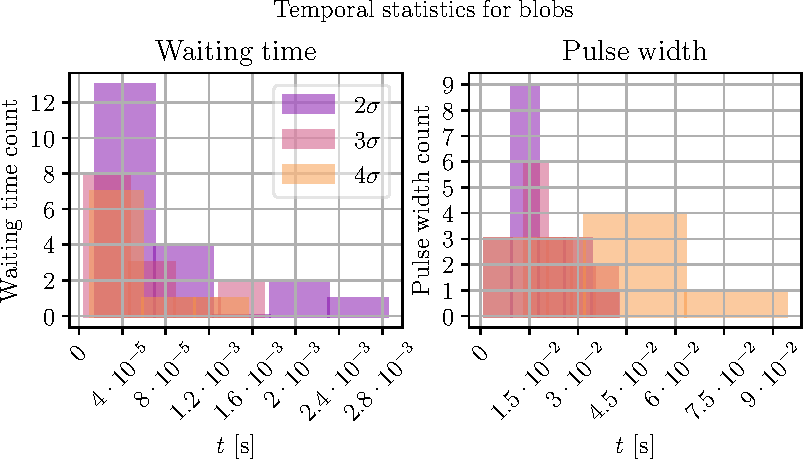
\includegraphics{fig/results/blobs/blobStatsB0_008Tweak}
    \end{center}
    \caption{
        Waiting times and pulse widths of $n$ for the conditional samples found for $B=0.08\T$.
    }
    \label{fig:tempStatBlob}
\end{figure}
